\chapter{总论}

\section{CT机的基本构造和原理}

1895年11月8日,德国著名物理学家威·康·伦琴(W.K.Roentgen)在一次阴极真空射线管放电实验中偶然发现了X线,它不仅是对物理学的巨大贡献,也为放射诊断学的创立和发展奠定了基础。100多年来放射诊断学获得了迅猛的发展。1969年英国物理学家G.N.Hounsfield利用人体对X线的吸收原理,结合计算机的图像重建和处理功能设计了计算机断层扫描机(computed
tomography,简称CT),这一成果于1972年向全世界宣告。这种图像质量好、诊断价值高的成像方法,使放射诊断学发生了重大突破,是对现代医学的卓越贡献。为此,Hounsfield获得了1979年诺贝尔医学生物奖。

\subsection{CT的发展简史}

1967年CT的基本组成部分即重建数学、计算机技术和X线探测器都已具备。那时,Hounsfield在EMI实验研究中心,从事图像识别和利用计算机存储手写字技术的研究。他证实了有可能采用一种与直接电视光栅方式不同的另一种存储方法,这种方法使信息检索更为有效。

首先,有人提议从三维物体的各个方向取读数。但后来的断层方法似乎更适用于图像重建和诊断。它意味着仅需从单一平面里获取透射的读数。因此,每个光束通路都可以看作联立方程中的许多方程之一,必须解这组联立方程才能获得该平面的图像。此原理用数学模拟法加以研究。然后经过反复实验,并用X线进行人脑组织标本扫描研究,于1969年Hounsfield设计成功CT机。第一个原型设备于1971年9月安装在Atkinson
Morley医院,1971年10月4日检查了第一个病人。在1972年4月英国放射学家研究年会上宣告EMI扫描机诞生了,接着在同年11月芝加哥的北美放射学会(RSNA)年会上向全世界宣布。1973年在英国放射学杂志上报道。1974年美国George
Town医学中心工程师Ledley设计了全身CT机,从此CT告别了只限于头颅检查的时代。1985年开发了滑环技术,1989年单方向连续螺旋型CT即螺旋CT的问世,是滑环技术的体现,是CT发展的重大突破。1991年开发了亚毫米扫描和双螺旋CT。1998年多层螺旋CT机问世,SIEMENS、GE、PICKER、TOSHIBA公司都相继生产。1983年超高速CT(ultrafast
CT,UFCT)又称电子束CT(electron beam technology
CT,EBCT)由美国Imatron公司率先研制成功,并于1993年推向市场。EBCT进一步开拓了CT的应用范围,例如心脏功能和形态学研究,心、脑、肾、冠状动脉的血流量测定等。2004年GE公司率先推出64层(64排探测器)螺旋CT,并在北美放射学会年会发布这一信息。此后SIEMENS公司亦研制出64层螺旋CT(探测器为40排,机架每旋转1周利用中间的32排探测器即可获得64层图像)。在2005年北美放射学会上,SIEMENS公司又推出了双源CT(SOMATOM
Definition),SOMATOM
Definition基于西门子64层螺旋CT的成熟技术,配备了两个同步旋转的X射线源、探测器,每组X射线源、探测器组合只需转动90\textsuperscript{o}
就可以获得质量很好的心脏图像;基于0.33s的机架旋转时间,它可获得83ms的时间分辨率,使心脏成像不受心率影响。

\subsection{CT机的基本结构和成像原理}

\subsubsection{基本结构}

1.X线发生系统:高压发生器、X线球管、冷却系统、前准直器(去除散射线,使X线呈束状排列)。

2.X线探测部分:探测器、模数转换器(将探测器形成的电信号转换成数字信号,输入计算机)、后准直器(去除被照物体后的散射线)。探测器分为气体和固体两大类。固体探测器由闪烁晶体构成,有碘化钠、碘化铯、钨酸镉、锗酸铋等;气体探测器采用气体电离室的原理,一般多用氙气。固体探测器灵敏度较高,但其几何利用率较低,而气体探测器则与之相反。

3.支架部分:扫描架和检查床。

4.计算机系统:第3、第4代CT机包括阵列处理机(图像处理计算机)和主计算机(中央处理系统)。

5.图像贮存、显示和记录部分:主要指磁盘(硬盘)、光盘、磁带或软盘、显示器和照相机等。

6.操作控制部分:主要指操作台的键盘。

\subsubsection{成像原理}

CT的成像原理与普通X线相仿,只是图像的载体用探测器代替了胶片或荧光屏。CT扫描时用高度准直的X线束扫描人体的某部位,并围绕该部位做360°匀速转动,穿过人体的X线再经过准直后,由探测器接受。探测器接受的大量信息经模数(A/D)转换器将模拟量转换成数字输入计算机,计算机计算出该断面上各单位体积的X线吸收值(CT值)并排列成数字矩阵。数字矩阵再经数模转换(D/A),用灰白不同的灰度等级在监视器荧屏上显示,就获得了该部位的横断解剖结构图像。不同密度的组织对X线的吸收量不同。探测器分辨X线量的敏感程度较X线透视和X线摄影高的多,其对组织的密度分辨力较常规X线检查约高10~30倍。

\subsection{CT机的分代}

CT机的发展通常以“代”来划分,主要依据X线球管和探测器的关系、探测器的数目、排列方式和两者的运动方式来划分。其实“代”并不完全反映CT机的性能优劣,即并非代数越高CT机性能越好,如第3、第4代CT各有其优点。

1.第1代CT机:X线为单射束,单个或数个探测器,运动方式为平移加旋转,扫描一层需数分钟,只能限于头颅扫描。

2.第2代CT机:它与第1代无质的区别。X线为小角度(3°~30°)扇形X线束,探测器从数个至几十个。运动方式仍为平移加旋转,扫描时间缩短至18秒左右。虽已扩大至全身应用,但运动伪影很明显,故实际仍限于头颅扫描。

3.第3代CT机:X线为角度较大(30°~45°)的扇形X线束,探测器也相应呈扇形排列,数目多达数百个。运动方式为旋转式,扫描时间一般为2~5秒,最快可达1秒,使CT检查应用于全身。滑环技术及随之应用的螺旋CT是第3代机型的重大突破。

4.第4代CT机:与第3代基本相同。探测器排列呈圆周状,固定在扫描架四周,仅为X线球管旋转。实际为第3代的变型,并无明显优越性,仅有少数厂家生产。

5.第5代CT机:即超高速CT机(UFCT),又称电子束CT(EBCT),与以前的CT机已有根本区别。采用电子枪结构,使每次扫描时间可缩短至30ms,大大有利于心脏CT扫描。

EBCT即UFCT,主要由电子枪、聚集线圈、偏转线圈、8排探测器群、台面高速移动的检查床和控制系统组成。采用电子枪发射电子束,经聚焦后由偏转线圈控制,使电子线旋转,并轰击四个平行的钨靶环,从而获得旋转的X线源,再采用8排探测器群来收集扫描数据。目前,扫描速度可达50ms。由于有4个靶环,一次可进行4次扫描,最快每秒可扫描24次,故对心脏、冠状动脉等心血管的研究有特殊的作用。它的优点是:①扩大了影像诊断范围;②提高了图像质量(减轻了运动伪影);③减少了造影剂用量,并提高了高峰显影质量;④增加了单位时间的检查人数;⑤可做血流量、血流速度和弥散等功能检查。

\section{CT的应用和进展}

\subsection{CT图像重建的常用数学演算方式}

通常使用的演算方式有:标准演算法(standard
resolution)、边缘演算法(edge resolution)和平滑演算法(smooth
resolution)等。可根据受检部位的组织成分及密度差异,选择合适的数学演算方式。标准算法适于分辨率要求一般的普通CT图像重建如头颅等。软组织演算法对密度差异很近的组织分辨率较好,常用于腹部脏器的检查。骨密度演算法的图像分辨率最佳,可以分辨密度差异很大的组织,适用于观察骨质及内耳、乳突等,也可用于肺部小病灶的高分辨率CT检查(HRCT)。

\subsection{影响CT成像的因素}

1.窗宽和窗位:形成CT图像的数字矩阵都是CT值,即组织密度的代表。空气的CT值约为-1000Hu,骨皮质的CT值约为1000Hu。而人眼大约能分辨16个灰阶。如果某幅图像内既含有空气,亦有骨皮质,则上下CT值范围约2000Hu差值,每个灰阶所包含的CT值范围为125Hu。那么,CT值相差在125Hu内的组织结构显示为同一灰阶(即同一灰度)而不能在CT图像上各自显示。所以就要在观察某幅图像或观察某部位的组织结构时,选择合适的CT值范围和该范围的中点,来观察或显示某幅图像,这一CT值范围即窗宽,其中点即为窗位。如观察脑组织窗宽为100Hu,窗位为35Hu;肺部窗宽为1000~1500Hu,窗位为-700Hu左右;纵隔窗宽为200~300Hu,窗位30~50Hu。

2.伪影与噪声:①伪影:在扫描中由于某种因素的影响而产生的被检物体不存在的假象。有机器因素造成的环状伪影、条状伪影、点状伪影等;亦有因人体内密度差异(例如骨骼、手术金属物、胃肠内钡剂)造成的伪影;还有运动性(如胃肠蠕动、呼吸、病人身体移动)伪影。扫描条件不当亦造成伪影。②噪声:分为光子噪声和组织噪声。前者亦称扫描噪声,即X线穿透人体后到达检测器的光子量有限,其在矩阵内各图像点(像素)上的分布不是绝对均匀所造成,以致均质组织或水在各图像点上的CT值不是相等的,为减少噪声需增加X线量。组织噪声为各种组织(如脂肪和脑组织)的平均CT值变异所致,即同一组织CT值常在一定范围内变化,以致不同组织可具有同一CT值。

3.部分容积效应:像素代表一个体积,此体积内可能含有各种不同组织。其CT值实际代表的是单位体积内各种组织CT值的平均数。例如骨骼和气体加在一起可以类似肌肉密度(CT值)。因此在较高密度区域中间的较小低密度灶的CT值常偏高,反之亦然。

4.空间分辨率与密度分辨率:前者是指影像中能显示的最小细节,后者是指能显示的最小密度差别。

\subsection{CT的检查方法}

\subsubsection{常用检查方法}

常用的CT检查方法有平扫描、增强扫描、动态CT扫描、靶扫描(亦称目标CT扫描、放大CT扫描)、高分辨率CT技术(HRCT)。

用于肝脏的特殊增强扫描即所谓的肝脏CT血管造影有两种方式,包括肝动脉插管的动脉造影CT(CTA)和经脾动脉或肠系膜上动脉注入造影剂的门静脉期扫描,又称经动脉门脉血管造影CT(CTAP)。

\subsubsection{特殊检查方法}

1.CT透视与实时螺旋CT扫描:其原理相同,即在接近0.6秒的延迟时间后CT图像以6帧/秒速度显示,能达到实时观察的目的。CT透视主要用于CT介入穿刺;实时螺旋扫描能在扫描期间评价增强程度、选择扫描时机等。

2.CT血管造影术:或称CT血管成像术(CT
angiography,CTA)是螺旋CT三维(3D)重建技术的应用结果,主要用于颈动脉、颅内动脉、胸主动脉、腹主动脉、髂动脉、肺动脉、肾动脉、肠系膜动脉及内脏静脉(如门静脉)成像。CT仿真内镜如CT胆管成像、泌尿系尿路成像等亦是螺旋CT三维重建的应用体现。

3.仿真内镜术(Virtual
endoscopy,VE):是将CT或MR获得的原始容积数据与计算机三维图像技术相结合,借助导航技术(navigation)或漫游技术(flythrough)以及伪彩技术来逼真的模拟腔道内镜检查的一种方法。于1994年Vining等首次报道应用于结肠CTVE。

目前CTVE主要用于:①气管和支气管;②鼻咽腔、鼻窦、喉和中耳;③胃和结肠;④大血管;⑤胆道;⑥肾盂、输尿管和膀胱;⑦脑室和椎管;⑧关节腔等。但它存在着不能显示病变的颜色、不能显示腔内扁平病变、定性能力差等缺点。目前虽处于初步认识阶段,但值得进一步深入研究。

4.CT灌注成像(CT perfusion
imaging):是指静脉注射造影剂的同时对选定的层面进行连续多次扫描,以获得该层面内每一像素的时间-密度曲线。根据该曲线利用不同的数学模型计算出血流量、血容量、对比剂的平均通过时间、造影剂峰值时间等参数,以此评价组织器官的灌注状态。它反映的是生理功能的改变,因此是一种功能成像,可用于了解脑、肝、肾、胰腺、心脏的灌注状态。灌注参数还能较准确的反映头颈部、肝、肾、胰腺和肺等部位的肿瘤内血管变化和血液动力学改变,对肿瘤的诊断及恶性肿瘤的分级有重要意义,且为治疗方案的选择提供有价值的信息。

5.CT定量骨密度测定:定量骨密度测定为骨矿物质含量测定的重要方法。其方法很多,如单光子吸收法和双光子吸收法等,其中以CT双效能定量测量法(定量CT法)比较可靠。

\subsection{常用的螺旋CT三维重建技术}

常用的三维重建技术有:多平面重建法(multi-planar
reformation,MPR)、最大强度投影法(maximum intensity
projection,MIP)、最小强度投影法(minimum intensity
projection,MinIP)、遮蔽表面显示法(shaded surface
display,SSD)、容积再现法(volume rendering,VR)以及曲面重建法(curved
planar reformation,CPR)、透明重建(Ray sum)等。

\subsection{应用和副反应}

\subsubsection{药理}

CT增强所用的造影剂主要为经肾脏排泄的含碘造影剂,但也有用硫酸钡制剂和胆道造影剂者。钡剂用于胃肠道检查;经肝脏排泄的胆道造影剂(包括口服和静脉用药)只用于胆道增强。

目前,CT检查使用的经肾脏排泄的造影剂多为水溶性造影剂,且均为三碘苯环的衍生物(图\ref{fig1-1})。根据其结构分为4型:①离子型单体:常用的有复方泛影葡胺、安其格纳芬(Angiografin);②离子型双聚体:常用的有碘卡明;③非离子型单体:常用的有优维显(碘普罗胺)、欧乃派克(碘苯六醇)、碘必乐(碘异酞醇)等;④非离子型双聚体:常用的有伊索显(碘曲仑)。

\begin{figure}[!htbp]
 \centering
 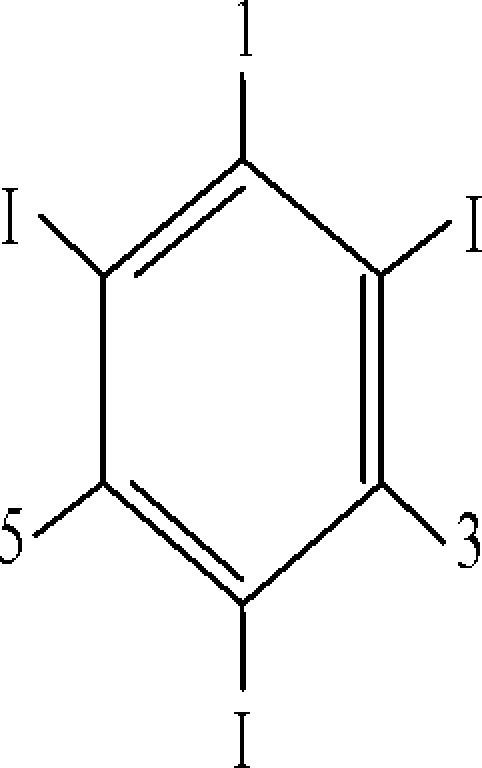
\includegraphics[width=.7\textwidth,height=\textheight,keepaspectratio]{./images/Image00002.jpg}
 \captionsetup{justification=centering}
 \caption{三碘苯环的基本分子式}
 \label{fig1-1}
  \end{figure} 

离子型者苯环上1位侧链为羧基盐(---COOR),具此结构的造影剂水溶性高,在水溶液中可离解成阴离子(含有三碘的苯环)及阳离子(葡甲胺、钠、钙、镁)。非离子型者苯环上1位侧链为酰胺衍生物(---CONH),其水溶性很高,但不离解于水中。单体造影剂是指一分子造影剂含有一个三碘化苯环,双聚体则有两个三碘化苯环。

经肾脏排泄造影剂的临床应用主要受下列因素影响:①碘浓度:与造影剂的增强效果有关。根据其浓度可分为4类:特高浓度(400mg/ml)、高浓度(350~400mg/ml)、中浓度(280~320mg/ml)、低浓度(80~240mg/ml)造影剂。特高浓度偶用于心脏、大血管造影和经静脉注射的动脉造影。中、高浓度造影剂尤其高浓度造影剂适用于快速静脉注射后的CT动态扫描。CT脑室或CT脊髓造影适用低浓度造影剂。②渗透压:高渗造影剂的副作用高于低渗造影剂;离子型渗透压高于非离子型;单体造影剂的渗透压高于双聚体者。③黏度:分子大、浓度高、温度低者黏度高。黏度越高给大剂量快速注射带来困难,且易形成微小血管的阻塞而引起局部的缺血缺氧。

\subsubsection{给药方式}

理想造影剂应具备以下条件:①显影清楚;②无毒、副作用;③易于吸收和排出;④使用方便;⑤性质稳定,易储存;⑥价格低廉。

除离子型造影剂碘卡明和非离子型造影剂优维显(碘普罗胺)、欧乃派克(碘苯六醇)、碘必乐(碘异酞醇)、伊索显(碘曲仑)可用于脑室及脊髓造影外,其他肾脏排泄造影剂禁用于脑室和椎管造影。因为这类造影剂容易进入蛛网膜下腔,可损害血脑屏障,引起抽搐及至死亡。

给药方式和用药量如下:

1.静脉团注法:亦称快速注射法。将某一剂量的高浓度造影剂加压快速注入静脉,在造影剂经血循环大量进入靶器官的供血动脉时开始CT扫描。这种方法可提供CT所需的高质量增强情况,现已成为常规增强方式。一般情况下造影剂用量为1.5~2ml/kg体重(成人一般注入80~100ml),注射流率为1~8ml/s。

2.静脉滴注法:以20~30ml/min的速度注入含碘量约为300mg/ml的造影剂100ml后,再行CT扫描的方法。

3.动脉注射给药法:主要用于肝脏肿瘤的诊断,即选择性注入肝动脉、脾动脉及肠系膜上动脉的CTA和CTAP扫描术,以0.7~1ml/s的流率注入70~100ml。

4.胆系造影增强:30ml胆影葡胺缓慢注射(大于5分钟)或100ml胆影葡胺静脉滴注给药(快速团注易引起严重副反应)。给药后30~60分钟达最佳强化。

5.蛛网膜下腔给药:由腰穿注入水溶性碘造影剂后做脊髓或脑室扫描。椎管造影浓度一般为200~300mg/ml,剂量10~15ml。脑室造影浓度为150
mg/ml,剂量5ml。

6.胃肠充盈造影:常用2%的碘水造影剂,用量无统一标准。①胃十二指肠检查前20~30分钟服500~800ml,上床前再服200~300ml。②小肠检查前2~3小时服800~1000ml以充盈结肠,检查前1~2小时服300~500ml以充盈小肠远端,检查前15~30分钟再服300~500ml充盈胃及小肠近端。③结肠检查一般灌肠注入1500~1800ml。

\subsubsection{含碘造影剂的副反应}

一般根据反应的轻重和需治疗的程度进行分类(见表\ref{tab1-1})。离子型和非离子型造影剂副反应发生率有明显差异,前者约为5%,后者约为1.3%,但后者重度反应明显少,约为0.01%
。所以对有肝、肾、心疾病、糖尿病、虚弱、恶病质和过敏体质者等高危人群尽可能选用非离子型造影剂。离子型和非离子型造影剂对肝肾功能的影响区别不大。

\begin{table}[htbp]
\centering
\caption{造影剂副反应的分类}
\label{tab1-1}

\includegraphics[width=\textwidth,height=\textheight,keepaspectratio]{./images/Image00003.jpg}
\end{table}

\subsection{CT的发展方向}

目前推出基于CT的肿瘤放疗系统即CT模拟定位系统,其软件、硬件专门为CT模拟设计制造,还配有立体定位介入引导系统,可帮助医师模拟和介入(活检或引流等),并配有组织间近距离放疗的CT立体定位机械手臂系统。

介入性CT可用于脑、肺、纵隔、肝、胰、肾、肾上腺、腹膜后淋巴结、盆腔肿块的穿刺活检及肿瘤治疗,亦可用于骨骼肌肉的穿刺活检。对胸腹部脓肿、腹部和盆腔囊肿(如肝、肾囊肿)进行穿刺引流、硬化治疗,其定位准确性更高。尤其对颅内血肿和脓肿的穿刺抽吸引流更具独到之处。在颈臂神经丛和腹腔神经丛神经阻断术中是其他影像学手段所不及。CT亦可用于植物神经阻断术。

\section{常用的CT技术术语}

\subsection{平扫描和增强扫描}

扫描(scan):CT机扫描架内的X线球管围绕人体旋转进行X线照射,探测器接收到衰减程度不同的X线,转换成电信号,输入计算机重建成图像,每旋转一次的动作称为扫描。

平扫描(simple
scan):不向血管内注射造影剂的一般扫描程序称为平扫。检查腹部虽然多口服造影剂以充盈胃肠,但仍叫平扫。

增强扫描(contrast enhancement
scan):即造影增强,以CE或+C表示。应用碘水造影剂注射入静脉或动脉内,使心血管、组织器官或病灶密度增加,有利于对病变或正常组织器官的显示。

\subsection{快速连续扫描和延迟扫描}

动态扫描(dynamic
scan):按设定的部位,自扫描起始位到终止位,自动地进行逐层扫描,扫描后自动处理并显示图像,可分为动床式和同层动态扫描。此种方法主要用于增强扫描。

快速连续扫描(fast continuous
scan):对感兴趣的某区,自动地进行多次快速扫描,了解器官功能活动情况、造影剂充盈与排泄情况,显示同一层次在不同时间的变化。实际属于同层动态扫描。

延迟扫描(delay
scan):部分病例需要在团注增强扫描结束后一段时间内再做病灶区域或整个脏器扫描。如疑肝血管瘤,可在团注造影剂后5~15分钟再做局部扫描,以观察病灶是否被造影剂充填。

\subsection{间隔扫描和重叠扫描}

薄层扫描(thin slice
scan):一般指层厚≤5mm的扫描。主要为了减少部分容积效应而进行此扫描。

间隔扫描(interval
scan):亦称间断扫描,即层距大于层厚的扫描。其扫描不是连续扫描,可以按一定间隔进行隔层扫描,减少了扫描层数。如层厚为10mm,层距为12mm、15mm、20mm,则为间隔扫描。

重叠扫描(overlap
scan):层距小于层厚的扫描。如层厚为5mm,而层距(间隔)为3mm,则为重叠扫描。

\subsection{定位扫描}

定位扫描(scan ogram)又称为topgraph或scout
view。即在X线球管固定时扫描出一幅人体正位或侧位像,用以做出扫描层次、方向、层距、间隔及扫描次数等计划。定位扫描像有时可代替普通X线片,供诊断参考。

\subsection{靶CT扫描}

靶CT扫描(target scan)亦称目标扫描(object scan)、放大扫描(magnify
scan),是针对某一感兴趣区做局部的CT扫描,即应用小显示野(DFOV)扫描。由于被显示的范围小而矩阵不变,在一定单位体积的区域内像素相对增多,故可明显提高空间分辨率。也可以在普通CT扫描结束后,利用收集的原始扫描数据做局部的靶图像重建。后一种方法因有扫描数据保存,故可做各种部位、大小和成像方式的图像靶重建。靶扫描或靶重建与CT图像的单纯放大不同。后者仅是把图像的某部分放大,并无从根本上改变像素的大小和成像方式,所以其分辨率未提高,其清晰度反而下降。

\subsection{螺旋扫描}

螺旋扫描(spiral scan or helical
scan)是建立在滑环技术上,是在一次数据扫描过程中X线管和探测器不停地向一个方向旋转(第4代CT机只是X线管旋转),检查床亦同时向前推进,整个扫描的轨迹呈螺旋形。故螺旋扫描采集的数据是某一器官的容积数据,因此重建时可以采用任意的重建距离来进行重建而获得相应的图像幅数。

在扫描过程中X线管每旋转一周,检查床推进的距离不一定要和层厚相等,检查床推进距离可以等于、大于或小于层厚。床推进距离和层厚之比称为螺距指数(pitch
index)简称螺距。螺距指数=床推进距离/层厚。床推进距离和层厚一致时螺距为1,床推进距离大于层厚时螺距>1,反之则<1。

\subsection{图像的重建和重组}

重建(reconstraction):是利用图像的原始数据来进行处理所形成的图像。

重组(refomatting):是利用已经形成的图像进行重新组合,如用来形成冠状面、矢状面、多平面(MPR)、三维(3D)图像。故重组与重建两者含义是有区别的,但多习惯于将重组亦称为重建。

\subsection{高分辨率CT技术}

高分辨率CT(hight resolntion
CT,HRCT)技术,即利用CT机具有的特殊软件,专为显示肺部弥漫性间质性病变以及结节病变等细微结构的重建方法,可使空间分辨率显著提高。一般采用1~2mm的薄层扫描,故亦可称为薄层高分辨率CT。实际上多采用骨密度演算法重建,所以也适用于观察骨质情况及内耳、中耳、鼻窦、眼眶等结构。

\subsection{窗功能和双窗}

窗宽(window
width):以W.W或W表示,即在观察某幅图像时所选择的CT值范围。观察不同的组织器官应选择合适的窗宽。

窗位(window level或window
center):以W.L、L或C表示,即所选择窗宽的CT值范围的中心值。

窗功能(window
function):即在观察某幅图像时,通过窗宽及窗位的调节,使所需观察的组织、器官及病变清楚显示称为窗功能。

双窗(dual
window):即为显示不同组织器官使用双窗位及双窗宽,具体数字在监视器或CT片上分别显示。例如胸部双窗显示,可在显示纵隔图像的同时,也显示肺的细节,有利于观察肺部病变与纵隔的关系。

\subsection{CT值及其换算公式}

CT值是指X线穿过人体后,探测器检测并换算出的组织、器官的衰减值,它所反应的是组织、器官的密度。其换算公式如下:

CT值=(μ组织-μ水)/μ水×α

μ组织为人体组织的吸收系数,μ水为水的吸收系数,α为分度因数。在换算时将水的吸收系数调节为1,空气的吸收系数为0,μ组织是相对水和空气而言的。α目前均采用Hunsfield的单位,其分度因数为1000,故水的CT值为0Hu,空气约为-1000Hu,骨的吸收系数最高可达水的两倍,即μ骨为2,故其CT值可高达1000Hu。最早的CT机采用EMI单位,其分度因数为500,故其CT值是Hu单位的一半,如空气为-500EMI单位。

\subsection{感兴趣区}

感兴趣区(region of
interest,ROI)即我们对图像某部分进行CT值测量分析的区域,其中有3项指示在画面上。

1.平均值(mean,m):即ROI内的CT值。

2.标准偏差(standard deviation,SD):即ROI内CT值的标准偏差。

3.面积(area,a):即ROI内的面积,以mm\textsuperscript{2} 表示。

\subsection{层厚和层距}

层厚(thickness or
slice)是指CT断层每个层面的厚度。层距(interval)是指每个扫描层面间的距离。根据层厚和层距的关系可分为连续扫描、间隔扫描和重叠扫描。

\subsection{像素和像体素}

矩阵(matrix):是一个数学概念,它表示一个横成行、纵成列的数字阵列。如320×320,512×512,1024×1024等。CT机将计算的人体断面各点的CT值以矩阵排列,构成分布图。矩阵由极小的方格所组成,其格数越多即矩阵越大,则显示的图像越清晰细致。

像素和像体素(pixel
voxel):一幅CT图像是由许多矩阵排列的小单元(小方格)组成,这些组成图像的基本单元称为像素。像素所表示的每一个小单元内具有一定宽度和一定厚度(层厚)的立方体称为像体素。体素是一个三维概念,而像素是一个二维概念,像素实际是体素成像时的表现,矩阵越大像素越小。

\subsection{周围间隙现象和伪影}

部分容积效应(partial volume
effect):亦称为平均值效应。每个像素的CT值为此像素或体素内各种物质CT值的平均值,故如果层厚过大,则一个像素内常含有两种或两种以上密度互不相同的物质,从而不能确切地反映其组织密度,这一现象称为部分容积效应。可通过减小层厚减轻部分容积效应的影响。

周围间隙现象(peripheral space
phenomenon):在同一层面内,与层面垂直的两个相邻且密度不同的物体,其物体边缘部的CT值不能准确测得,结果在CT图像上也不能清晰地分辨出两者的交界,这种现象亦称为边缘效应。

伪影(artifacts):由于某些因素的影响,图像中产生实际并不存在的各种形状的假象,称为伪影。

\subsection{空间分辨率和密度分辨率}

空间分辨率(spatial
resolution):又称高对比分辨率,是指CT对物体空间大小(几何尺寸)的分辨能力。通常用每厘米内的线对数或用可辨别最小物体的直径来表示。空间分辨率与被检物体的密度差别也有关,密度差别小则空间分辨率亦也相应减小。影响空间分辨率的主要因素为探测器的几何尺寸、探测器间的间隙和总的原始数据。重建算法也是影响空间分辨率的重要因素。

密度分辨率(density
resolution):又称低对比分辨率,是指CT对密度差别的分辨能力。以百分比表示,如密度分辨率为0.35%,即表示两个物质的密度差>0.35%时,CT即可将它们分辨出来。噪声和信噪比是影响密度分辨率的重要因素。

以上二者是相互制约的,空间分辨率与像素大小密切相关,一般为像素宽度的1.5倍。像素越小,数目越多,空间分辨率提高,图像越清晰,但在X线源总能量不变的条件下,每个单位容积所获得的光子数却按比例减少,使密度分辨率下降。

\subsection{“多层”和“多排”}

“多层”(multi-slice)和“多排”(multi-row)是两个完全不同的概念。1998年全球各相关公司相继推出了4层螺旋CT,然而不同的厂家采用了不同的探测器设计理念。如探测器的排列有对称和不对称之分,有8、16、34排不同的排列,但均为同步获得4层图像的扫描能力。2001年西门子公司率先推出了16层螺旋CT,而探测器的排列是24排。GE公司64层螺旋CT,为64排探测器;SIEMENS公司64层螺旋CT,探测器为40排,机架每旋转1周利用中间的32排探测器即可获得64层图像。故
“排”是指探测器的物理排列数目;而“层”是指数据采集系统同步获得图像的能力,即机架每旋转一周能够同步采集几层图像。所以,“多层螺旋CT”更加符合人们通常的理解且更趋合理。

\protect\hypertarget{text00009.html}{}{}

